\documentclass[12pt,letterpaper,noanswers]{exam}
\usepackage[usenames,dvipsnames,svgnames,table]{xcolor}
\usepackage[margin=0.9in]{geometry}
\renewcommand{\familydefault}{\sfdefault}
\usepackage{multicol}
\usepackage{wrapfig}
\pagestyle{head}
\definecolor{c03}{HTML}{FFDDDD}
\header{AM 22b Class 15}{}{Mar 5: probability}
\runningheadrule
\headrule
\usepackage{graphicx} % more modern
\usepackage{amsmath} 
\usepackage{amssymb} 
\usepackage{hyperref}
\usepackage{tcolorbox}

\usepackage[numbered,autolinebreaks,useliterate]{mcode}

\newcommand{\mb}[1]{\underline{#1}}

\begin{document}
 \pdfpageheight 11in 
  \pdfpagewidth 8.5in




% I need to review the torus trajectories...

\begin{itemize}
% \item There is a pre-class assignment (20 minutes of videos + a few WeBWorK exercises) due at 10am this Monday.  It is available on Canvas.
\itemsep0em
    % \item PSet 02 is due on Friday Feb 14th at 10am.
   % \item There is a pre-class assignment due Monday by 10am (pre-class 03).
    \item Problem set 05 is due on Thursday Mar 11th at 6pm.
    \item The Quiz 02 is available starting after class today.  Complete it by 6pm ET on Sunday.
    \item Skill check for C13, C14, C15 is on Monday.
\end{itemize}

\hrule
\vspace{0.2cm}

% partial derivatives, gradient
% local linearity, differential, directional deriv
% 2nd order partials + equations with partials

\noindent\textbf{Big picture}

This week we are studying integration for functions of multiple variables.  Today our focus is on triple integral practice and on probability.

\vspace{0.2cm}
\hrule
\vspace{0.2cm}

\noindent\textbf{Skill Check C15 Practice}
\begin{questions}
\question Let $p$ be the joint probability density function such that $p(x,y) = xy$ in the rectangle $R$ where $0\leq x \leq 2, 0\leq y\leq 1$.  $p(x,y) =0$ outside of the rectangle.  Set up an integral to find the fraction of the population such that $x+y \leq 2$.
\end{questions}


\vspace{0.2cm}
\hrule
\vspace{0.2cm}

\noindent\textbf{Skill Check C15 Solution}

The probability that $x+y \leq 2$ is given by $\int_S p(x,y)\ dA$ where $S$ is the region of $R$ in which $x+y\leq 2$.  $R$ is shown in blue, with $S$ plotted on top of it in red 

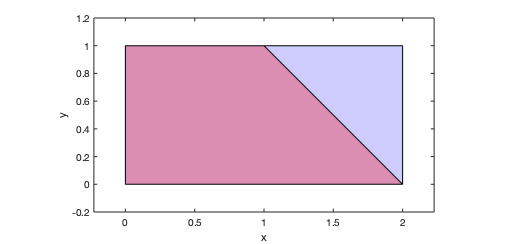
\includegraphics[width=3in]{img/C15skillcheck.png}

Setting up the integral:
\begin{align*}
   \int_0^1 \int_0^{2-y}xy\ dx\ dy
\end{align*}
If you were to integrate, you would find that the probability that $x+y\leq 2$ is less than half.

\vspace{0.2cm}
\hrule
\vspace{0.2cm}

\noindent\textbf{Teams}
You will work with this team on the in-class problems today.  Share something you hope to do this weekend.
\begin{multicols}{2}
1.  students here

\end{multicols}

%\vspace{0.2cm}
\hrule
\vspace{0.2cm}

\eject


\noindent\textbf{Probability for functions of a single variable.}
\begin{tcolorbox}
\begin{itemize}
\itemsep0em
    \item The function $p(x)$ is a \textbf{probability density function}, or pdf, if the fraction of the population for which $a\leq x\leq b$ $\displaystyle= \int_a^b p(x)\ dx$ with $\displaystyle\int_{-\infty}^{\infty}p(x)\ dx = 1$ and $p(x)\geq 0$ for all $x$.
    \item What does $\displaystyle\int_{-\infty}^{\infty}p(x)\ dx = 1$ mean in words?  This says that between $-\infty$ and $\infty$ you'll find the entire population.
    \item Why is $p(x)\geq 0$ for all $x$?  There is no interval where there would be a negative fraction of the population.
    \item $\displaystyle P(t) = \int_{-\infty}^t p(x)\ dx$ is the \textbf{cumulative distribution function.}. It gives the fraction of the population that has a value of $x$ below $t$.  $P$ is a nondecreasing function.  $\lim\limits_{t\rightarrow\infty} P(t) = 1$ and $\lim\limits_{t\rightarrow -\infty} P(t) = 0$.
    \item The fraction of the population having values of $x$ between $a$ and $b$ $\displaystyle= \int_a^b p(x)\ dx = P(b)-P(a)$.
\end{itemize}
\end{tcolorbox}

%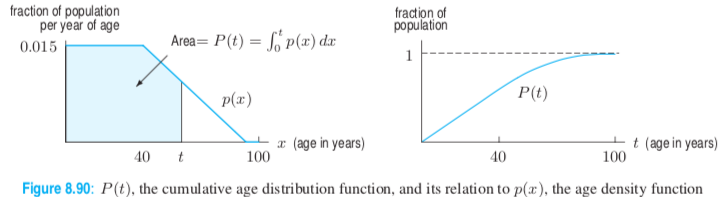
\includegraphics[width=\linewidth]{img/C20p8.png}


\noindent\textbf{Example (density and distribution functions)}. 

Match the graphs of the density functions, a,b,c, with the graphs of the distribution functions, I, II, III.  %\emph{pollQ}

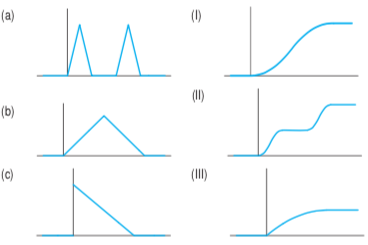
\includegraphics{img/C20p9.png}
\vfill

\eject

\noindent\textbf{Example: height of baseball players}

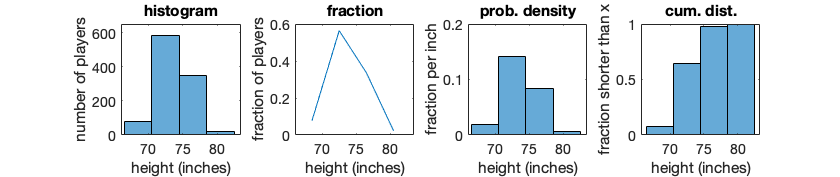
\includegraphics[width=\textwidth]{img/C14histbox4.png}

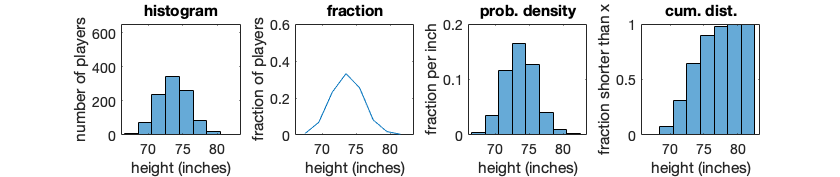
\includegraphics[width=\textwidth]{img/C14histbox2.png}

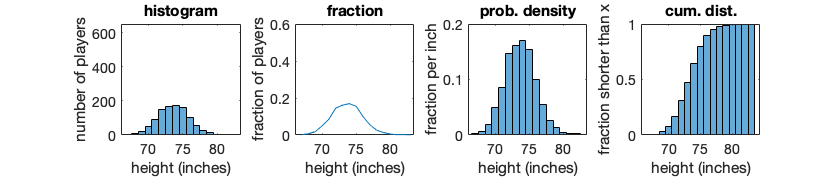
\includegraphics[width=\textwidth]{img/C14histbox1.png}


\begin{enumerate}
    \item Look at the first column (on the left).  What is changing between the different histograms? % Why is the number of players decreasing as you move down the rows?
    \item What about in the second column?
    \item What about in the third column?
    \item The shape of the plot is the same in the first column and in the third.  How would you convert from the values in the first to the values in the third?
    \item In the weight data on the next page, why does the histogram become "spiky" in the bottom row?
\end{enumerate}

\eject

\noindent\textbf{Example: weight of baseball players}

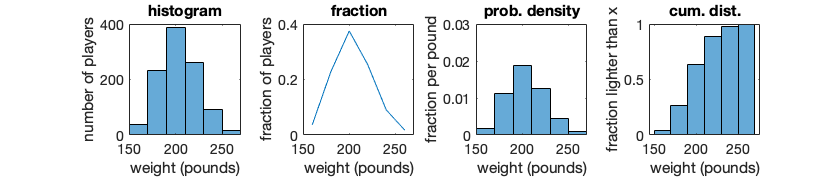
\includegraphics[width=\textwidth]{img/C14histboxweight20.png}

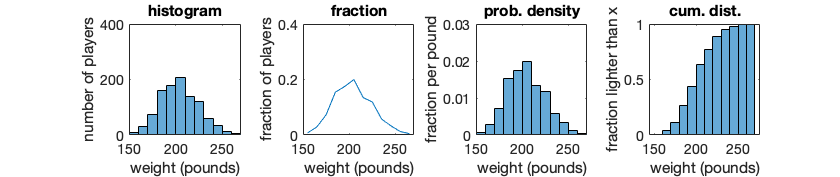
\includegraphics[width=\textwidth]{img/C14histboxweight10.png}

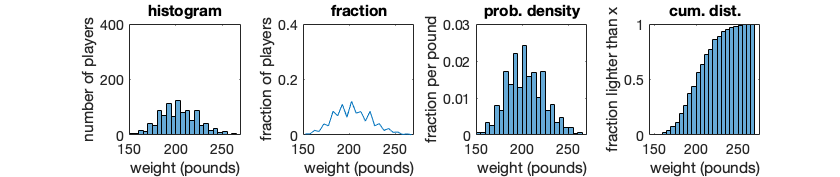
\includegraphics[width=\textwidth]{img/C14histboxweight05.png}

\vspace{0.2cm}
\hrule
\vspace{0.2cm}

\noindent\textbf{Joint probability} \S 16.6
\begin{tcolorbox}
\begin{itemize}
\itemsep0em
    \item A function $p(x,y)$ is called a \textbf{joint probability density function} or \textbf{pdf} for $x$ and $y$ if the fraction of the population that has $a\leq x\leq b$ and $c\leq y\leq d$ is given by $\int_a^b\int_c^d p(x,y)\ dy\ dx$ where $\int_{-\infty}^{\infty}\int_{-\infty}^{\infty} p(x,y)\ dy\ dx = 1$ and $p(x,y)\geq 0$ for all $x$ and $y$. 
    \item The probability that $x$ is falling in an interval of width $\Delta x$ around $x_0$ while $y$ is falling in an interval of width $\Delta y$ about $y_0$ is approximately $p(x_0,y_0)\Delta x \Delta y.$
  \item Two random variables are called \textbf{independent} when knowing the value of one variable does not give us any information about the distribution of the other variable.
\end{itemize}
\end{tcolorbox}


\vspace{0.2cm}
\hrule
\vspace{0.2cm}

\noindent\textbf{Example (joint probability distribution)}.
The plots below are showing information about the distribution of height and weight for major league baseball players.
The upper right graph, showing fraction per box area, is an approximation of the joint probability density function (pdf).  \\

Based on the pdf, are height and weight independent?



%\emph{pollQ}

\hspace{-0.5in}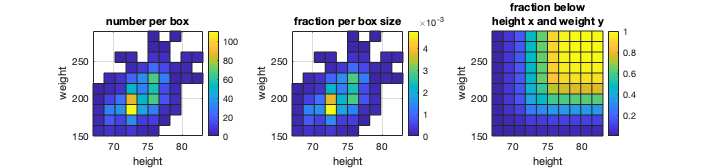
\includegraphics[width=0.9\linewidth]{img/C14joint.png}

\emph{They are independent if at each value of weight the height has an identical probability distribution and vice versa.}

%\vfill
%\eject



\vspace{0.2cm}
\hrule
\vspace{0.2cm}

\noindent\textbf{Example (joint probability distribution)}.
I generated $40000$ pairs of random numbers $(x,y)$ with $0\leq x\leq 1$ and $0\leq y \leq 1$.  Each number in the pair was drawn using a uniform distribution from the interval $[0,1]$.  I binned the numbers using $100$ boxes (a $10$ by $10$ grid).

\begin{verbatim}
data = rand(40000,2);
boxes = 10;
subplot(2,2,2)
histogram2(dat2(:,1),dat2(:,2),boxes,'normalization','pdf','DisplayStyle','tile')
xlabel('x'); ylabel('y'); title('fraction per box area')
set(gca,'fontsize',14)
caxis([0 2])
\end{verbatim}

An approximation for the joint probability density function (pdf) is shown on the upper right (it was make using the code given above).

Let $p(x,y)$ be the pdf.  $p(x,y) \approx k$ where $k$ is a constant.  Find an estimate for $k$.

%\emph{pollQ}

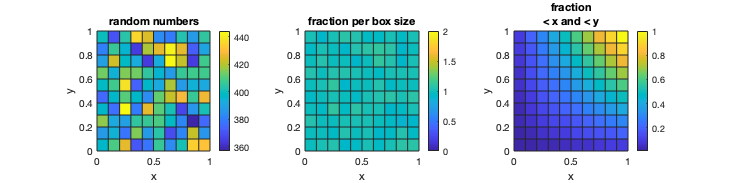
\includegraphics[width=\linewidth]{img/C14simulation.png}



\noindent\textbf{Example (probability density)}.  A point is chosen at random from the region $R$ in the $xy$-plane containing all points $(x,y)$ such that $0\leq x\leq 2, 0\leq y\leq 2$.  ``At random'' is being used to mean that the density function is constant on $R$.  

% The density is the fraction of points per unit area.

Which of the following is the joint probability density function?

\begin{oneparcheckboxes}
\choice $p(x,y) = 1/4$
\choice $p(x,y) = 1/2$
\choice $p(x,y) = 1$
\choice $p(x,y) = 2$
\end{oneparcheckboxes}



\vfill

\noindent\textbf{Example (probability)}.  For the joint probability density function and region $R$ above, what is the probability that we would choose a point such that $x > y$?

Shade the region in $R$ where $x>y$ to help you think about this.

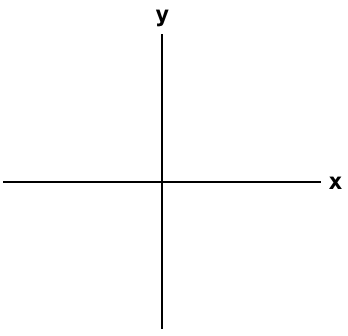
\includegraphics[height=1.5in]{img/C02axes-2.png}


%\emph{pollQ}


\eject

\vspace{0.2cm}
\hrule
\vspace{0.2cm}

\noindent\textbf{Quadrature} (not in text)
\begin{tcolorbox}
\begin{itemize}
\itemsep0em
    \item The term \textbf{quadrature} may refer to drawing a square with the same area as a given (planar) shape.  Example: `squaring the circle'.  \emph{Evidently `quadrate' means square}.
    \item \textbf{Quadrature} is also the term used to refer to finding an integral numerically.
    \item A \textbf{quadrature rule} determined by a set of nodes, $x_k \in [a,b]$, and a set of coefficients, $a_k$: $\displaystyle Q(f) = \sum\limits_{k=1}^n a_k f(x_k)$.  The \textbf{left Riemann sum} for approximating an integral, $\displaystyle Q(f) = \sum\limits_{k=1}^n \frac{1}{n}f(a + (k-1)h)$ with $h = \frac{b-a}{n}$,  is an example of a quadrature rule.  The \textbf{right Riemann sum}, $\displaystyle Q(f) = \sum\limits_{k=1}^n \frac{1}{n}f(a + h)$ with $h = \frac{b-a}{n}$, is another example.
    \item A quadrature rule for approximating an integral of a function $f$ has an associated \textbf{error}.  The error will depend on the properties of the function (specifically on its derivatives).
\end{itemize}
\end{tcolorbox}

\noindent\textbf{Example} (trapezoidal rule).

Consider $\int_0^1 f(x)\ dx$.  Write down a quadrature rule for approximating this integral.  Use the midpoint/trapezoidal rule, and use four even subintervals.
\vspace{1in}


\end{document}